% Laster inn pakker, kopiert og lim fra en MAT-INF dokument
\documentclass[11pt,english, A4]{article}
\usepackage[utf8]{inputenc}
\usepackage[T1]{fontenc}
\usepackage{babel}
\usepackage{amsmath}
\usepackage{amsfonts}
\usepackage{amsthm}
\usepackage[colorlinks]{hyperref}
\usepackage[onehalfspacing]{setspace}
\usepackage{bm,ltablex,microtype}
\usepackage{graphicx}
\usepackage{float}


\usepackage{fontawesome}

\usepackage{lmodern}

% ___________________NYTT DOKUMENT___________________
\begin{document}

% ______________EMNEKODE, FORFATTER OG PROSJEKTNAVN______________
\begin{center}
\Huge \textbf{Classification and Regression}\\
\Large{From linear and logistic regression to neural networks}\\
\vspace{6mm}
\small{FYS-STK4155: Applied data analysis and machine learning}\\
\small{Department of Physics, University of Oslo}

\vspace{6mm}
\Large {Mina Tangen and Tham Le}
\vspace{2mm}

% _____________________GITHUB-LINKEN____________________________
\faGithub\href{https://github.com/}{\  https://github.com/minatang1/project2} 


\thispagestyle{empty}
\end{center}

% _______________________DATO_______________________
\begin{flushright}
\small November, 2019
\end{flushright}
%\vspace{24mm}

% ___________________FORSIDEBILDE___________________
\begin{figure}[H]
  \includegraphics[width=\textwidth]{neurons}
  \caption{Biological neurons}
  \label{fig:biological neurons}
\end{figure}

\pagebreak
\newpage~\newpage

%___________________ABSTRACT______________________
\section*{Abstract}
ABSTRACT



\newpage


%_________________ CONTENTS________________
{
  \hypersetup{linkcolor=black}
  \tableofcontents
}

\newpage
%__________________INTRODUCTION____________
\section{Introduction}
Classification in statistical analysis is an important tool to identifying the outcomes in different situations and sort large amount of datasets. We want to know if the outcomes are predicted and classified right. Examples of classification problems includes to classify  a given physical state as solid or not, a pasient as healthy or sick or an e-mail as spam or not. In this project we study the challenges associated with classification and regression through implementation of logistic regression and the multilayer precepton (MLP). \\

The dataset we use for this project  is retrieved from UCI Machine Learning Repository and contains default payments from a bank in Taiwan (Yeh, I-C. \& Lien, C-H. (2009)). Our aim using this data set is to train a network, so that the explanatory variables $X_{i}$ are used to predict the response variable $Y$. Or, stated in more colloquial terms, we want to train our network to identify how a client's gender, age, education, previous payment history etc. can explain whether or not he/she pays their credit card bill on time. \

In the next section we will review methods such as logistic regression, stochastic gradient descent and multilayer precepton and their applications on the data set (Yeh, I-C. \& Lien, C-H. (2009)). Iin the following sections the results will 
be presented and discussed. Then, we will reach a conclusion in the last section. Additional equations, information about the dataset and code will be presented in the appendix. 






\newpage
%_____________________THEORY________________
\section{Methods}

%__________________________2.1 Logistic regression______________________________
\subsection{Logistic Regression}
\subsubsection{Binary classification and the Sigmoid function}
The logistic model classifies the observed data $x_i$ to be binary outcomes such as passed/failed, winning/losing, spam/not spam etc. Classification aims to predict the outcome correctly by finding patterns based on discrete variables. The probability that $x_i$ belongs to a category $y_i = (0,1)$ is given by the sigmoid function (Hjort-Jensen, M. (2019))
\begin{align}
f(x) = \frac{1}{1+\exp^{-x}}
\end{align}
and the probability of these two classes with $y_i$ either 0 or 1.

$$ p(y_{i} =1|x_i, \hat\beta) = \frac{\exp(\beta_{0} + \beta_{1}x_{i})}{1+\exp(\beta_{0} + \beta_{1}x_{i})}$$
$$ p(y_{i} =0|x_i, \hat\beta) = 1 - p(y_{i} =1|x_i, \hat\beta) $$
where $\hat\beta$ are the weights.

\subsubsection{Maximum likelihood and the cost function}

To find the total likelihood for all possible outcomes from the credit card dataset $D = {y_i, x_i}$, with the binary labels $y_i  = {({0, 1})}$ we can use the Maximum Likelihood Estimation (MLE). MLE is the product of the individual probabilities for every outcome $y_i$ (Hjort-Jensen, M. (2019)) defined as

\begin{align}
\qquad P(\mathcal{D}|\hat{\beta}) =\prod_{i=1}^n [p(y_i = 1| x_i, \hat{\beta})]^{y_i}[1-p(y_i = 1| x_i, \hat{\beta})]^{1-y_i} 
\end{align}
and from the negative log-likelihood function, we can obtain the cost function as

\begin{align}
-{P(\mathcal{D}|\hat{\beta})_{log}} = C(\hat\beta) = - \sum_{i=1 }^{n} {y_i({\beta}_0 + {\beta}_1x_i}) - log(1+\exp{\beta}_0 + {\beta}_1x_i)
\end{align}


%________________________2.2 Stochastic Gradient Descent Methods (SGD)___________________________
\subsection{Stochastic Gradient Descent Methods (SGD)}
To find the best possible fit for the dataset, we need to optimize the cost function $C(\hat\beta)$ by finding its minimum (Hjort-Jensen, M. (2019)). The SGD method is commonly used to achieve this. The general idea is that a function $F(x)$ decreases from x in a negative direction with negative gradient $- \nabla F({x}_i)$ where $\textit{x}$ are iteratively adjusted. The function is expressed as

\begin{align}
{x}_{i+1} = {x}_i - \eta\nabla F({x}_i)
\end{align}
with $\eta$ > 0.
The parameter $\eta$ is the learning rate, also the step length. It is important to choose a reasonable value for $\eta$, because small values will take longer time for SGD to converge or maybe not converge at all within the given time frame.  But for larger values SGD might pass the minimum or be too unstable to calculate.

% _________ IMAGE _____________
\begin{figure}[H]
  \begin{center}
  \includegraphics[width=10cm]{gradient_descent}
  \caption{Gradient descent algorithm visualized (Lanham, M. (2018)).}
  \end{center}
\end{figure}

%__________________________2.3 Multilayer precepton (MLP) ___________________________
\subsection{Multilayer precepton (MLP)}
A multilayer precepton is a feedforward artificial neural network (ANN) (Hjort-Jensen, M. (2019)). A precepton is a single neuron model that contributes to a larger neural network. The term \textit{multilayer} comes from having three or more layers in the network; an \textbf{input layer}, one or more \textbf{hidden layers} and an \textbf{output layer}.


% _________ IMAGE _____________
\begin{figure}[H]
  \begin{center}
  \includegraphics[width=9.5cm]{neural_network1.jpg}
  \caption{Visualizing of a neural network (Hassan, M.H. et al. (2015)).}
  \end{center}
\end{figure}



%_______ NEURON_______
\subsubsection{Neurons}
Artificial neurons are the building blocks of the neural network. These artificial neurons have the same mission as biological neurons, to receive a weighted input signal $\bm{x_i} \bm{w_i}$ and produce an output signal $\bm{y}$ by using the activation function $\bm{\sigma}$. 

% _________ IMAGE _____________

\begin{figure}[H]
\begin{center}
  \includegraphics[width=7cm,scale=0.5]{neuron}
  \caption{Artificial neuron (Chandra, L.A. (2012)).}
\end{center}
\end{figure}

%________________ Activation function__________________
\subsubsection{Activation function}
When the neuron receive the weighted inputs, the signal will pass through and reach the activation function. The function will map the weighted sum from the input to the output of the neuron. As mentioned, the activation function is a non-linear function. In this report the sigmoid function and ReLU were used. The mathematical model for the output signal is given as

\begin{align}
y = f\Big(\sum_{i = 1}^{n} = {w_i {x_i} + b_i}\Big) = f(z) 
\end{align}

The activation function receives the input signal $x_i$. The activation is defined as ${z} = (\sum_{i = 1}^{n} = {w_i {x_i} + b_i})$. The output y here is the input $x_i$ for the next layer. This connection does the multilayer precepton to a fully-connected neural network. 

To calculate the weighted sum we can take a look at the mathematical model for weighted sum in the first hidden layer

\begin{align}
z_i^1 = \sum w_{ij}^1 x_i = b_i^1 
\end{align}
And with a more general formal for the activation function, where $N_\ell$ is the number of neurons in layer $\ell$. 

\begin{align}
y_i^\ell = f^\ell(z_i^\ell) = f^\ell \Big(\sum_{j = 1}^{N_{\ell-1}} w_{ij}^\ell y_j^{\ell - 1} + b_i^\ell \Big) 
\end{align}

The are many activation functions in Machine Learning, but as mentioned, the Sigmoid function is the common function for logistic regression (section 2.1.1). The hyperbolic function and ReLU are also commonly used to train neural networks. The hyperbolic function is an alternative to the Sigmoid function and has a feature that lets the network learn
even when its initial weights are small values (Sussillo, d. \& Abbot, L.F. (2014)) because thanh'(x) is continuous around x = 0. While for Sigmoid and ReLu this can be problematic. The hyperbolic function 
\begin{align}
f(x) = tanh(x) = \frac{2}{1+\exp^{-2x}} -1
\end{align}

ReLU is short for Rectified Linear Unit and is the most common activation function in deep learning. ReLU is a non-linear activation function and are more efficiently for training large networks (Yang, J. (2017)). The formula for ReLU are

\begin{align}
f(x) = \begin{cases}
	  0,  &\text{for x < 0}\\
	  x,  &\text{for x $\geq$ 0}
	  \end{cases}
\end{align}

The following image show how the various activation function and their graph
%__________IMAGE____________-
\begin{figure}[H]
  \begin{center}
  \includegraphics[width = 5cm]{activation_functions}
  \caption{Activation functions and their graph (Jadon, S. (2018)).}
  \label{fig:activation_functions}
  \end{center}
\end{figure}



%__________________ Feedforward and backpropagation__________________
\subsubsection{Feedforward and backpropagation}
Now that we know how a neuron behaves and what an activation function does, we can explain the processes in a neural network; feedforward and backpropagation. Feedforward calculatse the predicted output \textbf{$\hat{y}$} for each neuron and backpropagation updates the weights and biases (Loy, J. (2018)).The following graph illustrates the processes 

\begin{figure}[H]
  \begin{center}
  \includegraphics[width = \linewidth]{nn_algorithm}
  \caption{Processes in a neural network (Loy, J. (2018)).}
  \label{fig:nn_algorithm}
  \end{center}
\end{figure}

As illustrated in figure \ref{fig:nn_algorithm}, the weighted input with bias $W_1x + b_1$ are coming in to the input layer. From the input layer, the signal goes through to the hidden layers and activate the activation functions $z = \sigma(W_1x+b_1)$) for every neuron (section 2.3.2) in the hidden layers. We get the total output signal in the last layer $\hat{y} = \sigma(W_{2}z+ b_2)$ and evaluate the model with the cost function $\hat\beta$ ($\textbf{Loss}(\hat y, y)$ in figure \ref{fig:nn_algorithm}). 

When we measured the error with the costfunction $C(\hat\beta)$ (section 2.1), we can now start to the process backpropagation. In order to adjust a reasonable value for the weights and bias. We use the the Stochastic Gradient Methods (section 2.2) to adjust the bias and weights.
 


%______________________________ONE HOT ENCODING ___________________________________
\subsection{One hot encoding}
Working with real data can be complicated if, for instance, the data is categorial data with variables that contain labels rater than numeric values. The numeric values might also not have a relationship between them. This is the case for the dataset we used in this project. By applying one hot encoding, the integer values representing a category for each featuer is being replaced by unique binary labels (0 and 1) for each of these values (see Implementation chapter).


%_________________________________Model evaluation _____________________________________
\subsection{Model evaluation}

% _________Confusion matrix___________
\textbf{A confusion matrix} is a table showing us how accurate our classification model is for the given dataset where the true values are known and gives us an insight into the errors (Brownlee, J. (2016)). 

% _________ IMAGE _____________
\begin{figure}[H]
  \includegraphics[width=\linewidth]{confusion_matrix}
  \caption{Confusion matrix (Namari, H. \& Shaffer, J. (2017).}
\end{figure}

\newpage
\textbf{Definitions of the terms}
\begin{itemize}
  \item True Negatives is the number of observations who is correctly predicted negative. 
  \item True Positives is the number of observations who is correctly predicted positive.  
  \item False Positives is the number of observed negatives who is predicted positive. 
  \item False Negatives is the number of observed positive, but is predicted negative. 
\end{itemize}

% _________Accuracy___________
\textbf{Accuracy} is defined as the ratio of true values who are correctly assigned by the model to the total number of observed values (Brownlee, J. (2016)). Accuracy can be defined by the equation following

$$ \text{Accuracy} = \frac{\text{True Positives + True Negatives}}{\text{total number of observations}}$$\\
The goal is to have a high accuracy, where the value 1 is the best. \\

% _________F1-score___________
\textbf{The F1-score} (or just F-score) is a measure of a test's accuracy, we need precision $p$ and the recall $r$ of the test to compute the F-score. The function reaches its best value at 1 and worst at 0.

Recall are defined as the ratio of correctly classified positive outcomes divides by the total number of positives (Brownlee, J. (2016). High value of recall indicates small number of False Negative, that means the dataset is correctly classified. 

$$ \text{Recall} = \frac{\text{True Positive}}{\text{True Positive + False Negative}} $$
\

Precision are defined as the ratio of correctly classified positive outcomes divided by the total number of originally positive input. High precision shows that positive outcomes is indeed positive, that means small number of False Positive.

$$\text{Precision} = \frac{\text{True Positive}}{\text{True Positive + False Positive}}$$
\\

\textbf{The $F_1$-score} is the harmonic mean of the precision and recall 

$$ F_1 = 2 \cdot{\frac{\text{recall} \cdot \text{precision}}{\text{recall} + \text{precision}}} $$\



% _________R2-score___________
\ \textbf{R2-score} measure the variance explained by the model divided by the total variance, and tell us how well the regression model fits the dataset by percentage from a scale 0 to 100 $\%$ (Tangen, M. \& Le, T. (2019)). 

\[
R^2(\hat{y}, \tilde{\hat{y}}) = 1 - \frac{\sum_{i=0}^{n - 1} (y_i - \tilde{y}_i)^2}{\sum_{i=0}^{n - 1} (y_i - \bar{y})^2},
\]
where $\bar{y}$ is the mean of the values.\\


%________MSE____________
\textbf{Mean Squared Error (MSE)} taking the average of the square of the values, where the values
is the differences between the observed values y and the predicted ones $\hat y$ . The bigger the values ii
the larger the error and 0 means that the regression model is perfect (Tangen, M. \& Le, T. (2019)). 

\[ MSE(\hat{y},\hat{\tilde{y}}) = \frac{1}{n}
\sum_{i=0}^{n-1}(y_i-\tilde{y}_i)^2, 
\] 



%_________________________________3 DATA _____________________________________
\section{Data}

%_______ Credit card data________
\subsection{Credit card data}
This dataset is retrieved from the Machine Learning Repository of the University of California, School of Information and Computer Science (Yeh, I-C. \& Lien, C-H. (2009)). It is a collection of payment data from a bank i Taiwan in 2005.


The dataset has 23 explanatory variables ($X_{1} - X_{23}$) in addition to client IDs and the response variable ($Y$). The explanatory variables holds information on the different consumers, such as information on their gender, age and education. The Appendix gives a detailed description of alle the explanatory variables. The response variable $Y$ describes whether or not the client defaults in the next month, i.e. if the client fails to pay by the deadline or not. $Y$ can have the value 1 (meaning that the client did fail to pay) or 0 (meaning that the client payed on time).

%_______Franke function_________
\subsection{Franke function}
The two-dimensional Franke function is a weighted sum of four exponentials. This function is commonly used for testing various fitting algorithms like we did in project 1 (Tangen, M. \& Le, T. (2019)). The function is following

\begin{align}
f(x,y) &= \frac{3}{4}\exp{\left(-\frac{(9x-2)^2}{4} - \frac{(9y-2)^2}{4}\right)}+\frac{3}{4}\exp{\left(-\frac{(9x+1)^2}{49}- \frac{(9y+1)}{10}\right)} \nonumber \\
&+\frac{1}{2}\exp{\left(-\frac{(9x-7)^2}{4} - \frac{(9y-3)^2}{4}\right)} -\frac{1}{5}\exp{\left(-(9x-4)^2 - (9y-7)^2\right) } \label{eq:Franke}
\end{align}


%______________________________IMPLEMENTATION__________________________________
\section{Implementation}

This project had three parts to implement: logistic regression, artifical neural network for classification and artificial neural network for linear regression. The artifical neural network we developed without using scikit-learn (and similair libraries) are reffered to sometimes in the results as ''NN'' and does at this point only have the option of 1 hidden layer.

\subsection{Data preprocessing}
As mentioned above, one should onehot encode the data when it represents different classes. 
We onehot-encoded columns 2, 3, 4, and 5, i.e. the gender, education, marital status and age columns. That is because the values in these columns do not have a set relationship between them. All columns holding information on payments always represent a month in between the different values, whereas the columns 2, 3, 4 and 5 does not have such a "set relationship"; there is not a month or another set number/meaning between graduate school and university, and university and high school for instance. \\

In addition, we removed invalid values and scaled the data (using scikit learn). We then used scikit-learn \textit{train\_test\_split} to split the data into training and test data. This function shuffles the data randomly before splitting. We ran our analyses using training and test sets of equals sizes, i.e. we used half of the data for training and the other half for testing. As our network performed poorly, we tried to increase the training amount, but this did not change the performance, as shown in figure \ref{fig:nn_conf_moretraining_acc0818} (compare with figures \ref{fig:nn_conf} and \ref{fig:mlp_conf}). It would have been interesting to create a more balanced data set, simply by taking out a number of 0s to make the distribution of 0s and 1s 50/50.

%___________Confusion matrix___________
\begin{figure}[H]
\begin{center}
  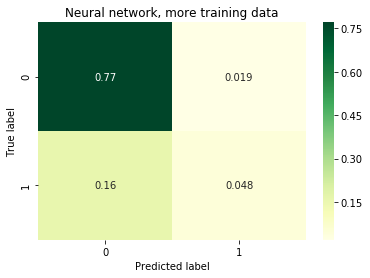
\includegraphics[width = 10cm]{nn_conf_moretraining_acc0818}
  \caption{Confusion matrix, more training data.}
  \label{fig:nn_conf_moretraining_acc0818}
  \end{center}
\end{figure}

\subsection{Evaluation metrics}

As ways of evaluating the performance of our network, we implemented the accuracy, F1, MSE and R2 scores using the scikit-learn library. In addition, we implemented the confusion matrix.

\begin{figure}[H]
  \begin{center}
  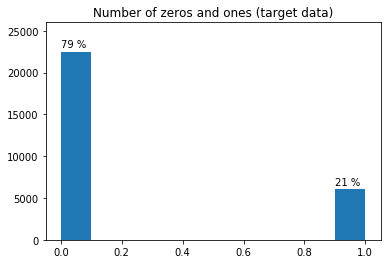
\includegraphics[width = 9cm]{pj2_distfig}
  \caption{Distribution of 0s and 1s in target data.}
  \label{fig:pj2_distfig}
  \end{center}
\end{figure}


As shown in the figure \ref{fig:pj2_distfig}, the targets of our dataset contains 79 \% 0s and 21 \% 1s. This means that even if our accuracy score is at 79 \%, the network might only have predicted only zeros (see figure \ref{fig:nn_conf_all0_acc0785}). Because of this imbalance in the dataset, the F1 score and confusion matrix are better at determining whether our network performs well or not. Early in the process of building our network we got decent accuracy scores, around $\sim 0.78$. However, when plotting the confusion matrix and F1 score, we discovered that the network only predicted one of the classes (0). The decent-looking accuracy score results from the fact that our dataset is very imbalanced. In this analysis, we have therefore focused mainly on the F1 score and confusion matrix to evaluate the network performance, as this takes imbalance into account. \\


We also applied a regularization parameter to our network, to make sure that the weights do not grow out of contol and overfit the training data.

The results from our own implemented neural network were compared to those of scikit-learns MLPClassifier.

We used the MSE and R2 scores to evaluate how the network did on linear regression. Since linear regression is not a binary classification problem, we had to change our model to output actual z values, rather than binary values. 



\newpage
%_________________________________ RESULTS _____________________________________
\section{Results \& discussion}

%______ Histogram av fordelingen________
%Figure (\ref{fig:pj2_distfig}) show the distribution of 0s and 1s in target data, we see that the data set is very imbalanced. Only 21\% is assigned to be 1s and 79\% is assigned to be 0s.


\subsection{Neural network}

As mentioned above, our network had issues of only classifying one category. To test if the network was actually learning, we trained it on a dataset only containing 0s and only 1s. We can see in figure \ref{fig:nn_conf_all0_acc0785} that the network was able to learn to classify both, which confirmed that the network was able to learn. To improve prformance, we then wanted to change the different hyperparameters.


%Figures (\ref{fig:nn_conf}) and (\ref{fig:mlp_conf}) shows confusion matrices for our own code for the Neural network and scikit-learns MLPClassifier (with the same hyperparamteres). As we can see, the results are similair, but not the best. The network is classifying many more 0s than 1s.


%___________Confusion matrix___________
\begin{figure}[H]
\begin{center}
  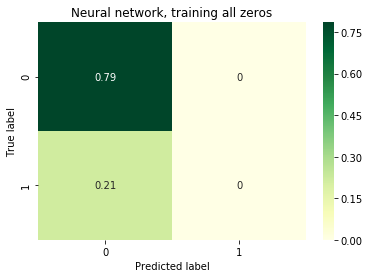
\includegraphics[width = 10cm]{nn_conf_all0_acc0785}
  \caption{Confusion matrix, only trained on 0s.}
  \label{fig:nn_conf_all0_acc0785}
  \end{center}
\end{figure}


%___________Confusion matrix___________
\begin{figure}[H]
\begin{center}
  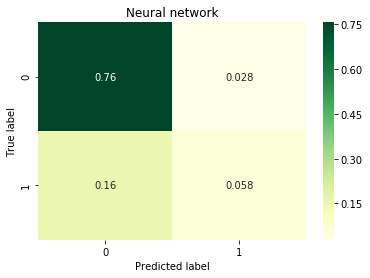
\includegraphics[width = 10cm]{nn_conf}
  \caption{Confusion matrix for neural network}
  \label{fig:nn_conf}
  \end{center}
\end{figure}


\begin{figure}[H]
\begin{center}
  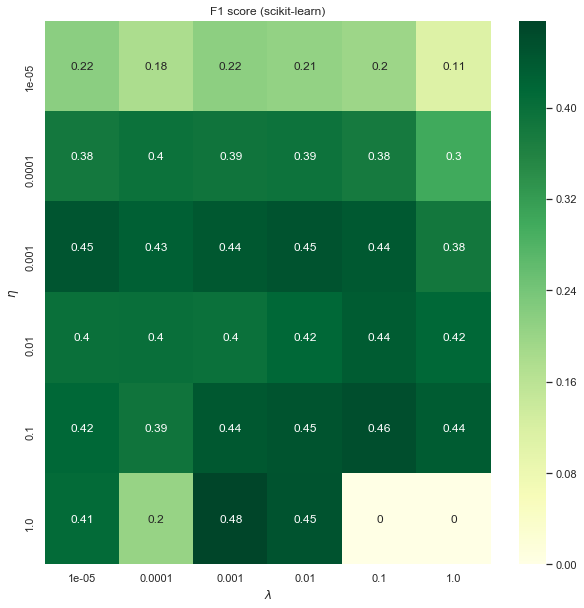
\includegraphics[width = 10cm]{f1_heatmap_sk}
  \caption{F1 score (MLPClassifier) as a function of $\eta$ (learning rate) and $\lambda$ (regularization)}
  \label{fig:f1_sk}
  \end{center}
\end{figure}


\begin{figure}[H]
\begin{center}
  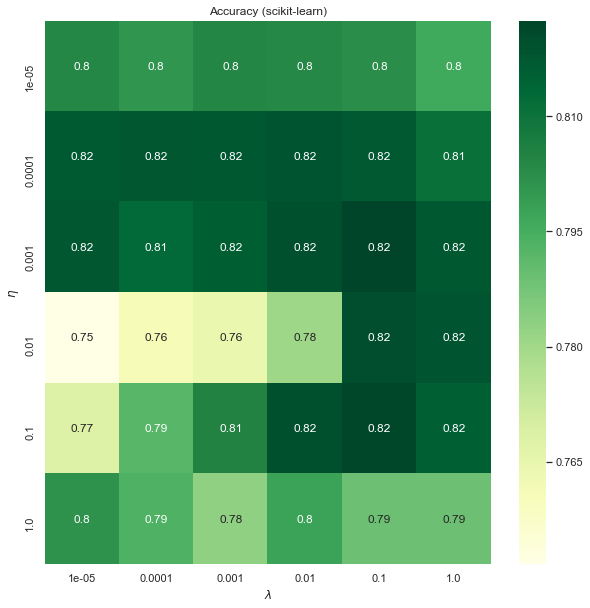
\includegraphics[width = 10cm]{acc_heatmap_sk}
  \caption{Accuracy score (MLPClassifier) as a function of $\eta$ (learning rate) and $\lambda$ (regularization)}
  \label{fig:acc_sk}
  \end{center}
\end{figure}

%___________Confusion matrix___________
\begin{figure}[H]
\begin{center}
  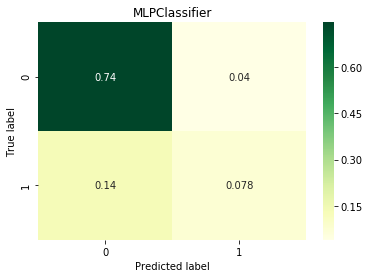
\includegraphics[width = 10cm]{mlp_conf}
  \caption{Confusion matrix for MLPClassifier}
  \label{fig:mlp_conf}
  \end{center}
\end{figure}

\begin{figure}[H]
\begin{center}
  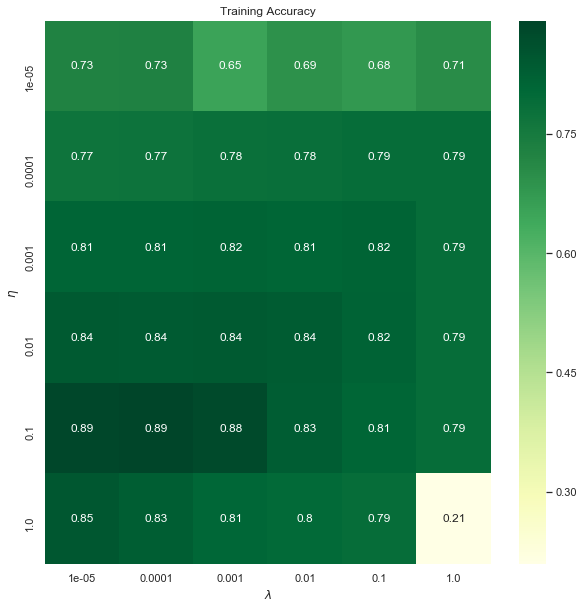
\includegraphics[width = 10cm]{training_acc_heatmap}
  \caption{Heatmap for test data}
  \label{fig:train_acc_heatmap (accuracy score)}
  \end{center}
\end{figure}

\begin{figure}[H]
\begin{center}
  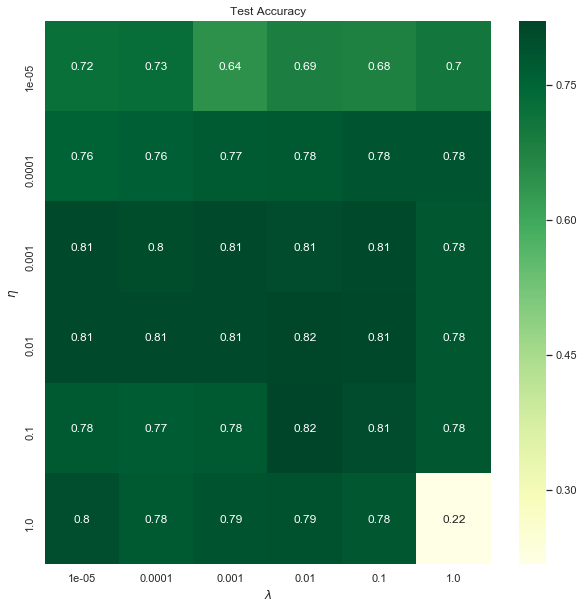
\includegraphics[width = 10cm]{test_acc_heatmap}
  \caption{Heatmap for test data (accuracy score)}
  \label{fig:test_acc_heatmap}
  \end{center}
\end{figure}

Figures \ref{fig:train_acc_heatmap} and \ref{fig:test_acc_heatmap} show how the accuracy score of our neural network changes with different sets of learning rates and regularization parameters. 

\begin{figure}[H]
\begin{center}
  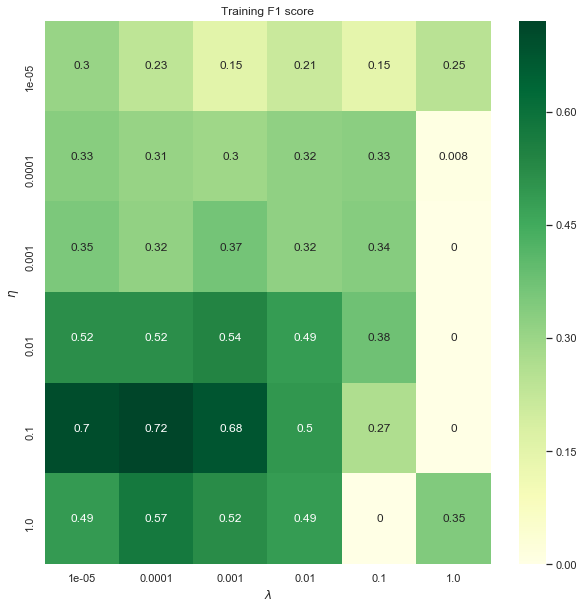
\includegraphics[width = 10cm]{training_f1_heatmap}
  \caption{Heatmap for test data (F1 score)}
  \label{fig:train_f1_heatmap}
  \end{center}
\end{figure}

\begin{figure}[H]
\begin{center}
  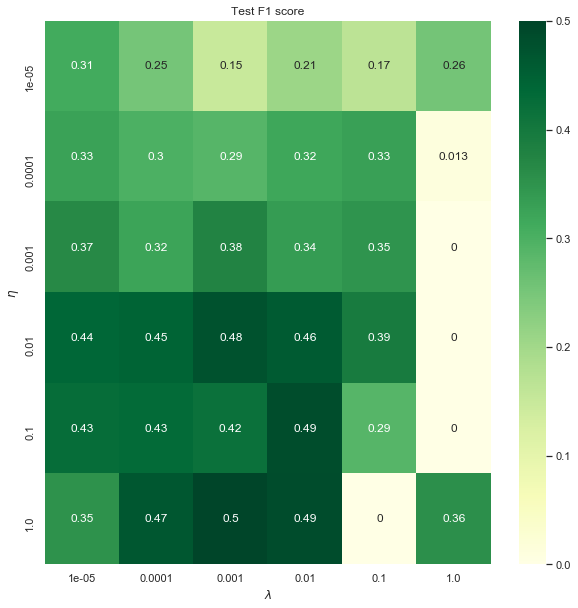
\includegraphics[width = 10cm]{test_f1_heatmap}
  \caption{Heatmap for test data (F1 score)}
  \label{fig:test_f1_heatmap}
  \end{center}
\end{figure}

Figures \ref{fig:train_f1_heatmap} and \ref{fig:test_f1_heatmap} show how the F1 score changes with different learning rates and regularization parameters.

\subsection{Franke's function}

Figures \ref{fig:mse_test_sklearn} and \ref{fig:mse_test_nn} shows the MSE score on the Franke function as a function of lambda and eta. As we can see, our implementation is performing much worse than that of scikit-learn, which might point to us having failed in changing the network to run for linear regression. There are, however, some combinations of lambdas and etas that yield good values. The same is evident when looking at the R2 scores (figures \ref{fig:r2_test_sklearn} and \ref{fig:r2_test_nn}).

\begin{figure}[H]
\begin{center}
  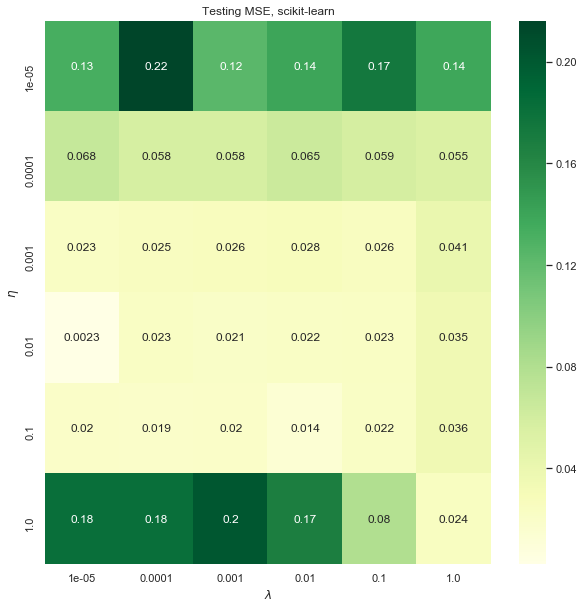
\includegraphics[width = 10cm]{mse_test_sklearn}
  \caption{Linear regression (scikit-learn), MSE as a function of $\eta$ (learning rate) and $\lambda$ (regularization)}
  \label{fig:mse_test_sklearn}
  \end{center}
\end{figure}

\begin{figure}[H]
\begin{center}
  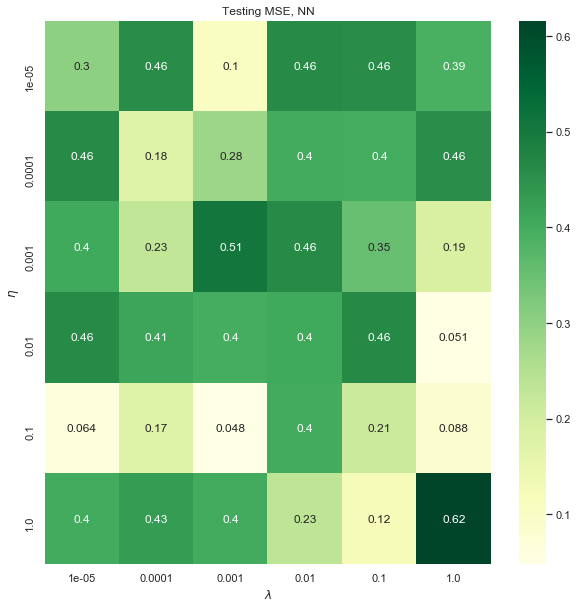
\includegraphics[width = 10cm]{mse_test_nn}
  \caption{Linear regression (NN), MSE as a function of $\eta$ (learning rate) and $\lambda$ (regularization)}
  \label{fig:mse_test_nn}
  \end{center}
\end{figure}

\begin{figure}[H]
\begin{center}
  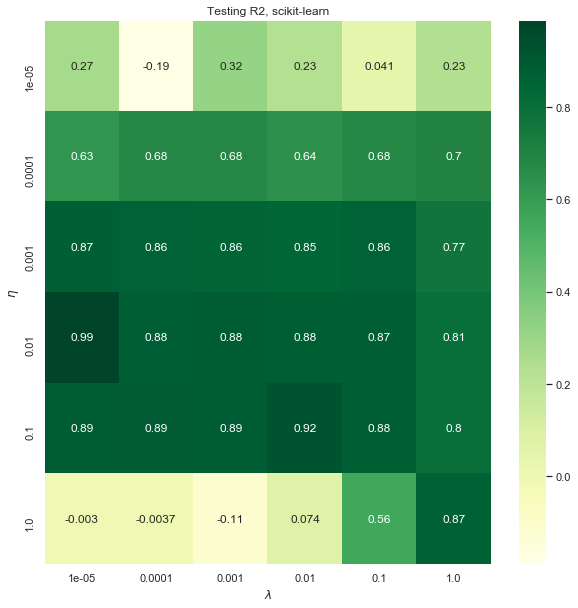
\includegraphics[width = 10cm]{r2_test_sklearn}
  \caption{Linear regression (scikit-learn), R2 as a function of $\eta$ (learning rate) and $\lambda$ (regularization)}
  \label{fig:r2_test_sklearn}
  \end{center}
\end{figure}

\begin{figure}[H]
\begin{center}
  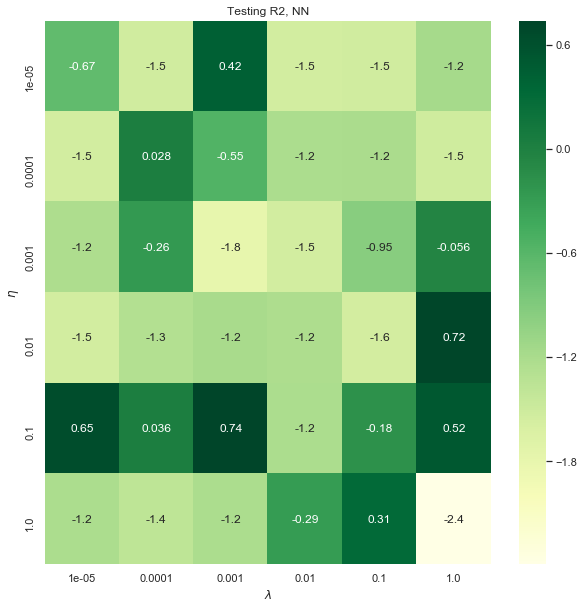
\includegraphics[width = 10cm]{r2_test_nn}
  \caption{Linear regression (NN), R2 as a function of $\eta$ (learning rate) and $\lambda$ (regularization)}
  \label{fig:r2_test_nn}
  \end{center}
\end{figure}

\begin{center}
\begin{table}
 \begin{tabular}{|c | c c c c c|} 
 \hline
 Metric & OLS & Ridge & LASSO & \textbf{Neural network} & \textbf{MLPRegressor} \\ [0.5ex] 
 \hline
$R^{2}$ & 0.9699 & 0.9699 & 0.628 & 0.74 & 0.99 \\ 
 \hline
 MSE & 0.0025 & 0.0090 & 0.0307 & 0.0484 & 0.0023  \\ [1ex] 
 \hline 
 \end{tabular}
 \caption{Regression metrics}
 \label{tab:reg_mets}
 \end{table} 
\end{center}

Table \ref{tab:reg_mets} shows the MSE and $R^{2}$ scores for the different regression methods Tangen, M. \& Le, T. (2019), and results produced in this project. As we can see, the MLPRegresor performs better than all other methods for regression. 


%________________________________ CONCLUSION ___________________________________
\section{Conclusion}

Our results agree with those from Yeh, I-C. \& Lien, C-H. (2009) for the classification case. We see a huge difference in performance of logistic regression and using neural networks. For the regression case, we see that the neural network from scikit-learn beats the other regression methods. \\

In the future, it would be interesting to try to improve our own neural network code, especially for the regression case, as it performed very badly. We suspect that there is an error we have yet to spot. From there, it would be interesting to see if we could make the network more flexible in terms of number of layers. It would also have been very intersting to compare the results if we were to make a dataset that was not biased, i.e. one containing the same amount of 0s and 1s in the target data. Our guess is that this would have helped the performance. Furthermore, we could have looked at different ways of preprocessing the data, in terms of one hot encoding and scaling of the data.

\newpage 
%_________________________________REFERENCES ___________________________________
\section{References}

Brownlee, J. (2016) \textit{What is a Confusion Matrix in Machine Learning}.\\
Downloaded from: https://machinelearningmastery.com/confusion-matrix-machine-learning/\\

Chandra, L.A. (2012) \textit{Perceptron: The Artificial Neuron (An Essential Upgrade To The McCulloch-Pitts Neuron}\\
Downloaded from: https://towardsdatascience.com/perceptron-the-artificial-neuron-4d8c70d5cc8d\\

Devore, J. L. \& Berk, K. N. (2012) \textit{Modern Mathematical Statistics with Applications} 2nd. ed. Springer. \\

Hassan, M.H. et al. (2015) \textit{Assessment of Artificial Neural Network for bathymetry estimation using High Resolution Satellite imagery in Shallow Lakes: Case Study El Burullus Lake}. Conference: Eighteenth International Water Technology Conference (2015).\\

Hjort-Jensen, M. (2019). \textit{Data Analysis and Machine Learning: Neural networks, from the simple perceptron to deep learning}. Lecture notes, FYS-STK4155 Applied data analysis and machine learning. University of Oslo.\\

Hjort-Jensen, M. (2019). \textit{Data Analysis and Machine Learning: Optimization and Gradient Methods}. Lecture notes, FYS-STK4155 Applied data analysis and machine learning. University of Oslo.\\

Hjort-Jensen, M. (2019). \textit{Data Analysis and Machine Learning: Logistic Regression}. Lecture notes, FYS-STK4155 Applied data analysis and machine learning. University of Oslo.\\

Jadon, S. (2018). \textit{Introduction on Different Activation Functions for Deep Learning}. 
Downloaded from: https://medium.com/@shrutijadon10104776/survey-on-activation-functions-for-deep-learning-9689331ba092\\

Lanham, M. (2018). \textit{Learn ARCore - Fundamentals of Google ARCore}. Publisher: Packt Publishing.\\

Loy, J. (2018). \textit{How to build your own Neural Network from scratch in Python}.\\
Downloaded from: https://towardsdatascience.com/how-to-build-your-own-neural-network-from-scratch-in-python-68998a08e4f6\\

Namari, H. \& Shaffer, J. (2017). \textit{Visualizing a Confusion Matrix}. 
Downloaded from: http://www.dataplusscience.com/VizConfusion.html\\

Sussillo, d. \& Abbot, L.F. (2014). \textit{Random Walk Initialization for Training Very Deep Feedforward Networks}. Conference: The International Conference on Learning Representations ICLR (2015).\\

Tangen, M. \& Le, T. (2019) \textit{Project1 FYS-STK4155}. University of Oslo, Oslo.\\

Yang, J. (2017). \textit{ReLu and Softmax Activation Functions}. \\
Downloaded from: https://github.com/Kulbear/deep-learning-nano-foundation/wiki/ReLU-and-Softmax-Activation-Functions\\

Yeh, I-C. \& Lien, C-H. (2009) \textit{The comparisons of data mining techniques for the predictive accuracy of probability of default of credit card clients}. Expert Systems with Applications, 36(2), 2473-2480.\\

\newpage

%_________________________________APPENDIX _____________________________________

\section{Appendix}


%_____________ Explanatory variables______________
\subsection{Explanatory variables}


%____________table_____________
\begin{table}[H]
   \centering
   %\begin{center}
   \begin{tabular}{ c | c | c | c} \label{tab:EXPVar}
   Variable & Description & Unit / value range & Name\\
   \hline
   $X_{1}$ & Given credit & NT dollars & LIMIT\_BAL\\
   $X_{2}$ & Gender & 1 - 2 & SEX \\
   $X_{3}$ & Education & 1 - 4 & EDUCATION \\
   $X_{4}$ & Marital status & 1 - 3 & MARRIAGE \\
   $X_{5}$ & Age & Year & AGE \\
   $X_{6} - X_{11}$ & History of past pay & -1, 1 - 9 & PAY\_1\footnote{NOTE: In the original dataset, $X_{6}$ was named    PAY\_0, but we changed it to PAY\_1 to avoid being confused} - PAY\_6 \\
   $X_{12} - X_{17}$ & Amount of bill statement & NT dollars & BILL\_AMT1 - BILL\_AMT6 \\
   $X_{18} - X_{23}$ & Amount of previous payment & NT dollars & PAY\_AMT1 - PAY\_AMT6
  \end{tabular}
  %\end{center}
  \caption{Overview of explanatory variables of the Credit card data set}
\end{table}

\textbf{Variable $X_{1}$} holds the amount of credit (given in NT dollars), and includes both the individual and supplementary credit (i.e., the consumers own credit and the credit of the family of that consumer).\\
\textbf{Variable $X_{2}$} describes the gender, and has a value of 1 if the consumer is male and 2 if the consumer is female.\\
\textbf{Variable $X_{3}$} describes the consumer's level of education, and takes on values from 1 to 4, where 1 is graduate school, 2 university, 3 high school and 4 others.\\
\textbf{Variable $X_{4}$} describes wether the consumer is married ($X_{4} = 1$), single ($X_{4} = 2$) or some other marital status ($X_{4} = 3$).\\ 
\textbf{Variable $X_{5}$} holds the age of the consumer in years.\\
\textbf{Variables $X_{6} - X_{11}$} holds past monthly payment records, from April ($X_{11}$) to September ($X_{6}$) 2005. These variables take on values from 1-9, which describes the delay of the past payment in months. E.g., if one of the variables has value 1, then the payment was done one month after the deadline and 9 months (or more) if the variables has the value 9. If the payment was done on time, these variables has value -1.\\ 
\textbf{Variables $X_{12} - X_{17}$} holds the amount on the bill statement (given in NT dollars) for the same months as for the previous variables, whereas variables $X_{18} - X_{23}$ holds the amount of the previous payments (given in NT dollars), also for those same months. As for the past monthly payment records, the variables are orderer backwards (starting in September ($X_{12} / X_{18}$) going to April ($X_{17}/X_{23}$)).





\end{document}